% ===========================================
% SYLLABUS
% Written by: Braidan Duffy
%
% Date: 12/27/2022
% Last Revision: 12/28/2022
% ============================================

\documentclass[
	letterpaper, % Page size
	fontsize=10pt, % Base font size
	twoside=true, % Use different layouts for even and odd pages (in particular, if twoside=true, the margin column will be always on the outside)
	%open=any, % If twoside=true, uncomment this to force new chapters to start on any page, not only on right (odd) pages
	%chapterentrydots=true, % Uncomment to output dots from the chapter name to the page number in the table of contents
	numbers=noenddot, % Comment to output dots after chapter numbers; the most common values for this option are: enddot, noenddot and auto (see the KOMAScript documentation for an in-depth explanation)
]{kaobook}

% Choose the language
\ifxetexorluatex
	\usepackage{polyglossia}
	\setmainlanguage{english}
\else
	\usepackage[english]{babel} % Load characters and hyphenation
\fi
\usepackage[english=british]{csquotes}	% English quotes

\usepackage[]{outlines}

\usepackage{color, soul} % Enable text color changes and highlighting

\usepackage{cancel}

\usepackage[]{pdfpages}

\usepackage{diagbox}

% Load packages for testing
% \usepackage{blindtext}
%\usepackage{showframe} % Uncomment to show boxes around the text area, margin, header and footer
%\usepackage{showlabels} % Uncomment to output the content of \label commands to the document where they are used

% Load the bibliography package
\usepackage{kaobiblio}
% \addbibresource{bibliographies/learning_materials.bib} % Learning Materials bibliography file
% \addbibresource{bibliographies/main.bib} % Bibliography file

% Load mathematical packages for theorems and related environments
\usepackage[framed=true]{kaotheorems}

% Load the package for hyperreferences
\usepackage{kaorefs}

\usepackage{authblk}

\usepackage{listings}

\usepackage{xcolor}

\graphicspath{{../images/}} % Paths in which to look for images

\makeindex[columns=3, title=Alphabetical Index, intoc] % Make LaTeX produce the files required to compile the index

\makeglossaries % Make LaTeX produce the files required to compile the glossary
\newglossaryentry{computer}{
	name=computer,
	description={is a programmable machine that receives input, stores and manipulates data, and provides output in a useful format}
}

% Glossary entries (used in text with e.g. \acrfull{fpsLabel} or \acrshort{fpsLabel})
\newacronym[longplural={Frames per Second}]{fpsLabel}{FPS}{Frame per Second}
\newacronym[longplural={Tables of Contents}]{tocLabel}{TOC}{Table of Contents}

 % Include the glossary definitions

\makenomenclature % Make LaTeX produce the files required to compile the nomenclature

% Reset sidenote counter at chapters
%\counterwithin*{sidenote}{chapter}

\usepackage{xcolor}
% \definecolor{codegreen}{rgb}{0,0.6,0}
% \definecolor{codegray}{rgb}{0.5,0.5,0.5}
% \definecolor{codepurple}{rgb}{0.58,0,0.82}
% \definecolor{backcolour}{rgb}{0.95,0.95,0.92}
% \lstdefinestyle{mystyle}{
%     backgroundcolor=\color{backcolour},   
%     commentstyle=\color{codegreen},
%     keywordstyle=\color{blue},
%     numberstyle=\tiny\color{codegray},
%     stringstyle=\color{codepurple},
%     basicstyle=\ttfamily\footnotesize,
%     breakatwhitespace=false,         
%     breaklines=true,                 
%     captionpos=b,                    
%     keepspaces=true,                 
%     numbers=left,                    
%     numbersep=5pt,                  
%     showspaces=false,                
%     showstringspaces=false,
%     showtabs=false,                  
%     tabsize=2
% }
% \lstset{style=mystyle}

\usepackage{multirow}

\renewcommand{\arraystretch}{1.3}

\begin{document}

\pagelayout{wide} % Remove margins

% -------------------FRONT MATTER-------------------

% \titlehead{Version 1}
% \subject{Florida Institute of Technology: OCE2901}

% \title{Surf Engineering Analysis Syllabus}
% \subtitle{Spring 2023}

% \maketitle

% -------------------MAIN CONTENT-------------------

\chapter*{OCE2901 Syllabus}

\paragraph*{Instructor:} Braidan Duffy, bduffy2018@my.fit.edu

\section*{Course Description} \labsec{course_desc}
This course is designed to teach students the fundamentals of data collection and analysis through a series of field-intensive experiments.
Students will learn how to design an experiment given a research question, deploy and work with instruments in the field, offload data, and write analysis scripts to understand variable relationships.
Students will demonstrate their problem-solving abilities during student-led deployments and will be expected to operate without instructor intervention.

The students will be broken into two research teams.
Graduate and undergraduate students will be evenly dispersed between the teams, with the former expected to take on leadership and mentorship roles.
Graduate students will be expected to perform more complex analyses and drive their groups to success while also teaching their younger colleagues the basics of data analysis, field experimentation, and technical writing.
Undergraduate students will be expected to help with the analysis and field experimentation design and execution. One or two may be asked to take on a higher responsibility within the team. 

This course is \emph{not} a programming course.
There will be programming involved in the field reports and homework assignments.
Fundamentals will not be extensively covered so it is up to the individual student to study programming in their own time or seek help from their more-knowledgeable peers.

\subsection*{Meeting Times} \label{meeting_times}
\subsubsection*{Lectures}
Monday, Wednesday, Friday; 10:00-10:50 (0h50min)\\
Spring 2023, January 9 - May 5\\
Crawford 230

\subsubsection*{Office Hours}
Monday, Wednesday, Friday; 13:00-15:00\\
Or, by appointment (preferred)\\
Link 156

\subsubsection*{Field Experiments}
We will be meeting (hopefully) every week in the field once field data collection begins. 
Dates and times are to be determined by each group individually for their respective weeks. See the Field Experiments section.

\textbf{Location:} Howard E. Futch Memorial Pack at Paradise Beach, Melbourne, FL, 32903 \\
\href{https://goo.gl/maps/tjdfqDwxHv3FmtNz8}{Google Maps}

\subsection*{Objectives \& Outcomes} \label{ssec:objectives_outcomes}
The objectives of this course are to teach students techniques in field data collection and data analysis, as well as a basic understanding of water waves and the physics behind surfing - including force balances, buoyancy, and hydrodynamic drag.
\textbf{Students will not learn how to surf.}
Instead, they will be taught how surfing can be used as a tool to collect data by programming specialized instruments, deploying them, and then recovering and analyzing the data they gather.

This course shall:
\begin{enumerate}
    \item Provide the students with experience needed to solve engineering problems through direct measurement by learning instrument deployment, data collection, and analysis techniques,
    \item Teach students how to design a field experiment given available, recordable data, and a research questions,
    \item Teach students how to draw conclusions from relationships present in the field data they analyze.
\end{enumerate}

Upon successful completion of the course, the student shall be able to:
\begin{enumerate}
    \item Identify common terminology used in data analysis,
    \item Design a field data collection experiment given available parameters and a research question
    \item Determine the important variables for solving research-based problems,
    \item Explain and apply basic physics in a marine setting,
    \item Discuss properties and characteristics of water waves relating to time series analysis,
    \item Understand the methods of data processing and error handling,
    \item Qualitatively and quantitatively describe the coastal wave environment,
    \item Deploy and retrieve instruments from the coastal surf zone,
    \item Analyze field data using time-series analysis techniques such as spectral analysis and filtering.
\end{enumerate}

\subsection*{Target Audience \& Prerequisites} \label{ssec:target_audience_prereqs}
On the undergraduate side, this course is intended for students who are interested in learning how to design field experiments and begin the fundamentals of data analysis.
Undergraduate students are not required to have any prior experience with programming or wave mechanics, but it will certainly help.
If you are taking the wave mechanics course in conjunction with this course, you will gain an appreciation of the practical side to wave mechanics while simultaneously learning the fundamentals.

On the graduate side, this course is designed for students that have some experience running field experiments, programming and data analysis.
While none of these are strictly necessary to have before taking the course, they are extremely important as you will be responsible for managing, motivating, and mentoring the undergraduate students on your team and in the class.
Therefore, you will need to have the initiative to learn the skills you may be lacking with respect to this course. 
Teams are expected to be able to operate autonomously and your ability to do so will directly correlate with your team's success.
In addition, more demanding tasks will be asked of you on homework assignments and the field reports.

\textbf{Course pre-requisites:} PHY1001 - Physics 1

\subsection*{Course Resources} \label{ssec:course_resources}
The course material will be regularly updated on \href{https://fit.instructure.com/}{Canvas} and \href{https://github.com/Legohead259/OCE2901-Material} {GitHub}. The GitHub repository will have all of the supplementary and study material required by students. The Canvas page may also contain these files, but GitHub will be the most up to date.

Students will be \emph{required} to purchase the following text books:
\begin{itemize}
    \item \footnotemark Karimpour, A., FUNDAMENTALS of DATA SCIENCE with MATLAB. 2020, ISBN-10: 1-7352410-1-6, ISBN-13:978-1-7352410-1-2
    \item Karimpour, A., OCEAN WAVE DATA ANALYSIS, Introduction to Time Series Analysis, Signal Processing, and Wave Prediction, 2018, ISBN-13: 978-0-692-10997-7
\end{itemize}
\footnotetext{for students without previous MATLAB experience}

\paragraph*{Recommended Readings} Students are not required to purchase these particular textbooks or reference guides, but the following are recommended:

\begin{enumerate}
    \item Emery, W.J. and Thompson, R.E., Data Analysis Methods in Physical Oceanography, 2nd Edition, Elsevier, 2004.
    \item Butt, T. and Russell, P., Surf Science, University of Hawaii Press, 2002
    \item CEM (Coastal Engineering Manual) US Army Corps of Engineers.
    \item Dean, R.G. and Dalrymple, A., Water wave Mechanics for Engineers and Scientists. World Scientific, 1991.
    \item Munson, Young, Okiishi, and Huebsch, Fundamentals of Fluid Mechanics, 7th edition, John Wiley \& Sons (or similar)
\end{enumerate}

\section*{Grading Policies} \labsec{grading_policies}
This course covers several student performance metrics: (i) Reports, (ii) Exams, (iii) Assignments, and (iv) Participation. The weighting for these metrics is below:

\begin{table*}[ht!]
    \begin{tabular}{l | c}
        \toprule
        \multicolumn{1}{c|}{\textbf{Metric}} & \textbf{Weight} \\
        \midrule
        Reports         & 60\% \\
        Exams           & 20\% \\
        Assignments     & 10\% \\
        Participation   & 10\% \\
        \bottomrule
    \end{tabular}
\end{table*}

Students will be assigned the following letter grade and GPA quality points based on their weighted sum assignment scores according to the following:

\begin{table*}[h!]
    \begin{tabular}{c | c | c}
        \toprule
        \textbf{Score} & \textbf{Letter Grade} & \textbf{Quality Points} \\
        \midrule
        90-100              & A     & 4 \\
        80-89               & B     & 3 \\
        70-79               & C     & 2 \\
        60-69\footnotemark  & D     & 1 \\
        <60                 & F     & 0 \\
        \bottomrule
    \end{tabular}
\end{table*}
\footnotetext{Undergraduate students only. \textbf{Graduate students will fail below a 70.}}

\pagebreak

\section*{Course Schedule} \labsec{course_sch}
\begin{table*}[h!]
    \labtab{course_sch}
    \begin{tabular}{ c | p{0.3\linewidth} | p{0.3\linewidth} | p{0.3\linewidth} }
        \toprule
        \textbf{Week} & \multicolumn{1}{c|}{\textbf{Monday}} & \multicolumn{1}{|c|}{\textbf{Wednesday}} & \multicolumn{1}{|c}{\textbf{Friday}} \\
        \midrule
        01/09   & Syllabus and Introduction         & Variables and Surfing             & Physics of Surfing and Waves      \\
        01/16   & \textbf{NO CLASS}                 & Experimental Design               & Data Analysis and Acquisition     \\    
        01/23   & Instrument Introduction           & Field Data Collection Basics      & Data Processing Techniques        \\
        01/30   & Data Processing Techniques        & How to Design a Field Experiment  & Field Experiment Dry Run          \\
        02/06   & Python Basics for Data Processing & MATLAB Basics for Data Analysis   & Group 1 - Wave Tank Wet Run       \\
        02/13   & Downloading and Preparing Data    & Structuring an Analysis Script    & Group 2 - Wave Tank Wet Run       \\
        02/20   & Dimensional Analysis              & Statistical Methods and Errors    & Group 1 - Field Deployment 1      \\
        02/27   & Pressure Data Analysis - WBW      & Pressure Data Analysis - Spectral & Group 2 - Field Deployment 1      \\
        03/06   & Time Series Techniques - Theory   & Time Series Techniques - Practice & Group 1 - Field Deployment 2      \\
        \hline
        03/13   & \multicolumn{3}{c}{\textbf{SPRING BREAK (NO CLASS)}}                                                      \\
        \hline
        03/20   & Fourier Transform Explained       & Wave Characteristics              & Group 2 - Field Deployment 2      \\
        03/27   & Multi-Dimensional Analysis        & Filtering and Windowing           & Group 1 - Field Deployment 3      \\
        04/03   & Dynamics and Reference Frames     & Sensor Fusion for Attitude        & Group 2 - Field Deployment 3      \\
        04/10   & Relating Different Datasets       & Work Day                          & Group 1 - Field Deployment 4      \\
        04/17   & Correlation and Regression        & Work Day                          & Group 2 - Field Deployment 4      \\
        04/24   & Discussion of Testing Thetis      & Reflection on Class and Data      & \textbf{STUDY DAY (NO CLASS)}     \\
        \hline
        05/01   & \multicolumn{3}{c}{Final Oral Presentation on the Beach (Bring Food and Games)}                           \\
        \bottomrule
    \end{tabular}
\end{table*}

\section*{Assignment Schedule} \labsec{assignment_sch}
\begin{table*}[h!] 
    \labtab{assignment_sch}
    \begin{tabular}{ l | c }
        \toprule
        \multicolumn{1}{c|}{\textbf{Assignment}} & \textbf{Due Date} \\
        \midrule
        Homework 1: Variables and Sensors List                      & January 11    \\
        Homework 2: Research Topic Quad Chart                       & January 16    \\
        Homework 3: Dice Roll Assignment                            & January 20    \\
        Literature Review Quad Chart\footnotemark[2]                & January 27    \\
        Field Experiment Procedure                                  & February 03   \\
        Homework 4: Data Plotting                                   & February 10   \\
        Experiment Schedule                                         & February 20   \\
        Latest Experimental Procedure Draft                         & 24 Hours Before Deployments \\
        Risk Management Assessments                                 & During Deployments \\
        Deployment Checklist                                          & After Deployments \\
        Deployment Report                                           & 2 Weeks After Deployments \\
        Midterm                                                     & March 24 \\
        Final Report                                                & April 26 \\
        Final (Oral Presentation)                                   & May 05 \\
        \bottomrule
    \end{tabular}
\end{table*}
\footnotetext[2]{Graduate students only}

\section*{Other Important Dates} \labsec{other_dates}
\begin{table*}[h!]
    \labtab{other_dates}
    \begin{tabular}{ l | c }
        \toprule
        \multicolumn{1}{c|}{\textbf{Event}} & \textbf{Date} \\
        \midrule
        Last day to drop \emph{without} a "W"  & January 18 \\
        Last day to drop \emph{with} a "W"     & March 24   \\
        \bottomrule
    \end{tabular}
\end{table*}

\section*{Team Definition} \labsec{team_def}
Students will be separated into two groups for this course.
They will be given the option to elect which group they want to be in using a public sign up form.
Students that have not voluntarily joined a group by the end of the first day of class shall be randomly assigned a group.
Once groups have been finalized, \emph{there will be no appeals for reassignment except for consequential reasons (e.g. harassment, bullying, stalking, or other forms of malfeasance that would require instructor/administrative interference)}.
The onus is on the students to learn how to work together to complete their research tasks.

\subsection*{Research Question} \label{ssec:research_question}
Each group will be given the option to come up with their own research question they would like to explore.
The question can be anything desired by the team, but it must conform to the following:
\begin{enumerate}
    \item Be related to surfing and wave dynamics
    \item Be quantifiably answered given instruments currently accessible to the course or student
    \item Be deep enough to facilitate research over the entire semester
    \item Be quantifiably answered by using appropriate data analysis techniques
\end{enumerate}
If, by the due date of the Research Topic Quad Chart, students do not have a research topic to propose, one shall be given to them. 
This shall not incur a point penalty as the grade will be forgiven.

\paragraph*{Default Research Question} How can we relate the surfer motion to the wave dynamics using three unique dimensionless parameters?

\subsection*{Team Composition} \label{ssec:team_comp}
Each team will be broken into four roles in a hierarchy shown in Figure \ref{fig:team_structure}: the Principal Investigator (PI), Technician, Safety Coordinator (SC), and Research Assistants.
There will be one student for each of the executive roles (PI, Technician, SC), and all the rest will be Research Assistants.
Graduate Students are required to fill the executive roles.
If there are less than three graduate students in a team, then an undergraduate may take either the Technician or SC roles.
If there are more than three graduate students, then those that do not have an executive role will be Research Assistants and expected to do the bulk of the mentoring and high-level data analysis.

\begin{figure}
    \caption{Hierarchy for each research team}
    \labfig{team_structure}
    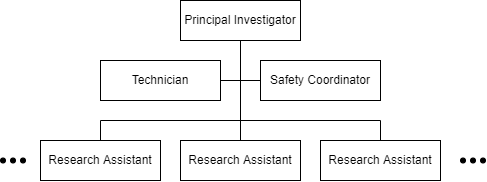
\includegraphics[width=5.0in]{team_structure.png}
\end{figure}

\paragraph*{Principal Investigator} The Principal Investigator, or PI, is responsible for the team organization, submissions, task delegations, and broader research objectives.
This person shall be the driving force pushing the team towards the successful conclusion of their research as well as making sure all team members are equally involved in the process.
All training, managing, and coordination shall be run through the PI.

\paragraph*{Technician} The Technician is the team member that is primarily responsible for the proper care and maintenance of the equipment used during field deployments.
They will also be responsible for the transportation, deployment, and recovery of the instruments in the field.
They should be omniscient with all of the pieces of equipment and able to diagnose, troubleshoot, and fix any errors that the instruments encounter.
Additionally, the Technician will need to train all the other team members on their duties such that experiments can still be performed in their absence (\emph{hint:} this is critical for the midterm assignment!)

\paragraph*{Safety Coordinator} The Safety Coordinator, or SC, is the member primarily responsible for the team's safety during field deployments.
This means properly caring for, maintaining, stocking, and carrying the team's first aid kit as well as being responsible for the field safety procedures.
They are also responsible for setting the watch on the beach to ensure swimmers and surfers are always being monitored.
Before deployments, the SC is expected to lead a safety brief with the team and perform a Risk Management Assessment.
During deployments, the SC will also be responsible for the conduct of team members on the beach so that no one is injured and risks are mitigated.
As a result, the SC \emph{cannot} be a surfer or swimmer during the field deployments.

\paragraph*{Research Assistant} The Research Assistants have only the responsibility given to them by the executive roles.
They can be responsible for portions of the data collection, preparation, and/or analysis process.
This is expecting to be mostly undergraduates so their responsibilities should reflect whatever skills they possess or whatever skills they wish to acquire/improve upon.

\section*{Field Experiments} \labsec{field_experiments}
Every week starting on the seventh week of the course (February 20), each group will go out to the field to collect data.
Before this point, students will have created a schedule for when each experiment will occur (see Experiment Schedule assignment).
However, while making that schedule, each group should consider several factors:

\begin{enumerate}
    \item The time of ideal surf conditions (i.e. low tide, offshore winds, waves about 2-3 feet)
    \item The time all of the group members can meet
    \item The time the instructor(s) can meet at the beach
    \item The time any external surfers (e.g. students from the surf club) can meet at the beach 
\end{enumerate}

When there is a field experiment, the class will not meet for a normal lecture.
The group that is running the experiment and the instructor(s) will meet at the beach to collect data.
The other group is invited to join so long as they do not interfere or interrupt the other group's experiment.
Otherwise, it is highly encouraged to use these days as work and research days.

\subsection*{Before the Experiment}
At least 24 hours before the scheduled experiment time, the Principal Investigator shall upload the latest revision of the group's experimental procedure to the appropriate Canvas assignment (or the instructor's email if Canvas is not available).
This latest document should highlight the changes made from the previous version (i.e. color the new text red, as opposed to black), as well as have a detailed contribution list from each team member and their responsibilities.
The instructor shall review the document and either approve or deny the group's experiment.

If the experimental procedure is denied, the group must rework it based on feedback from the instructor and resubmit it.
If the group still does not have a procedure approved by the time of the experiment, they will be forced to postpone the data collection until their next available opportunity.

\subsection*{During the Experiment}
At the start of the experiment, the PI and SC will lead a team briefing.
The PI shall inform each team member what their roles and responsibilities are and ensure that members are comfortable and knowledgeable with their roles.
The SC shall then conduct a safety review through a Risk Management Assessment (see the RMA handout).
The SC has the ultimate say over the data collection - if they feel that the conditions are unsafe or someone is about to get hurt, they are expected to cancel the experiment.

\subsection*{After the experiment}
A detailed field deployment report is expected two weeks after the deployment concludes.
All team members should be responsible for, and contribute, to a portion of the report.
This should all be documented in a separate document submitted with the report.
The team should also reflect on how the experiment was conducted and modify their experimental procedure to reflect lessons learned or successes.
These changes should be highlighted for the instructor to note during the next procedure review.

\paragraph*{Failure To Perform Duties} If group members fail to perform their duties, the penalties shall be applied to the entire team.
The PI is ultimately responsible for ensuring every team member is contributing and fulfills their obligations.
If a student is overloaded, it is expected that the PI finds a way to reduce their load.
Conversely, if a research assistant or other member is struggling, then it is expected that they report their problems to the PI so that it can be managed.

If a team member is chronically neglecting the team or their duties, it is up for the PI to approach the instructor about the issue.
Students who do not contribute to their team face dismissal from the course, or an automatic failure.
If there are any questions or doubts, do not hesitate to contact the instructor.
The penalties for missing sections or contributions will be up to the discretion of the instructor; the more you communicate with the instructor, the easier it will be for them to make a judgement that is amiable to everyone.

\section*{Course Policies} \labsec{course_policies}
\subsection*{Attendance} \label{ssec:attendance}
Attendance is \textbf{\emph{mandatory}} as the course is based on extensive field data collection requiring the presence of all students. 
Successful completion of this course will require students to travel to the beach regularly for meetings, and to come prepared with knowledge of their role and responsibilities ahead of time.
Students are expected to contribute to their teams both before, during, and after field deployments as discussed with the team's Principal Investigator.

\subsection*{Online Course Management} \label{ssec:course_mgmt}
This course will be published in the online learning tool, \href{https://fit.instructure.com/}{Canvas}, and will be made readily available to all students. 
Canvas provides an online cross-platform solution for students and instructors to engage and will handle all of the assignment submissions and \emph{preliminary} grades for students.
Assignments will be issued and submitted through the Canvas platform and students will be expected to submit the required documents by the due date and time listed on the assignment submission box.
If, for whatever reason, assignments are unable to be turned in through Canvas, they must be emailed to the instructor and timestamped by the date and time established.

Grades will also be posted on Canvas for students to track their progress in status in the course.
However, there is no guarantee that the posted grade in Canvas will represent the final course grade submitted to the registrar, nor may it be up-to-date if grade corrections are necessary.
In the event a student is not satisfied by their grade posted in Canvas, they are more than welcome to schedule a \emph{face-to-face} meeting with the instructor to discuss.
Emailed requests to change grades may be considered but it will be more effective to meet with the instructor in-person to ensure the change is made properly.

Canvas will also have a "Files" section where students can find relevant course resources and documents to aid in their studies.
Students may request certain documents be uploaded to Canvas to share with their classmates and they may download all files freely if they wish to have their own local copies.
The Canvas may be periodically updated to reflect changes or addendums to course content, but it may not necessarily reflect the most up-to-date information.
For the most updated course material, please consult the class \href{https://github.com/Legohead259/OCE2901-Materials}{GitHub Repository}. \emph{You may be surprised what you find in there...}

\paragraph*{Late Work Policy} Late work will be accepted with a penalty up to five (5) days after the assignment due date.
Starting one minute after the deadline passes, 10\% will be deducted from the assignment grade.
Every 24 hours after that will be another 10\% until the fifth deduction.
At that point, the assignment will no longer be accepted and the grade will be an irremediable 0.
If the assignment is a group assignment, \emph{all members} will receive the same penalty irregardless of if their individual contributions were submitted on time.

Exceptions and extensions may be granted on a case-by-case basis by the instructor.
\emph{Communicate, communicate, communicate}.

\paragraph*{Remote Learning} The COVID-19 pandemic has radically changed the learning environment we are in.
The traditional ideology of in-person, all the time, has been fundamentally destroyed by two years of remote working.
As the pandemic has lessened, Florida Tech has resumed in-person classes, full-time.
However, the benefits of remote and asynchronous learning cannot be understated to those that can effectively learn that way, or need to for whatever reason.

Therefore, the class will be taught with a hybrid option.
Lectures, projects, and assignments will be primarily done in-person in accordance with Florida Tech policies and instructor preferences but, students will have the option to perform assignments or attend lectures remotely.
There will be a Zoom link that will be active for all of the class lectures; lecture presentations and classes will be recorded and uploaded to Panopto.
However, students will be required to attend field deployments and the final presentation, barring significant reasoning.
These absences must be accompanied by a written excuse from the Office of the Dean of Students in accordance with the excused absence policy.
Students must inform the instructor of any intent to attend remotely ahead of the planned date.

\subsection*{For Students with Handicaps and/or Disabilities} \label{ssec:accommodations}
Students with handicaps and/or disabilities will be given special considerations depending on their condition and Florida Tech policy. Please meet with the instructor privately to discuss any concerns or arrangements. 

\subsection*{Academic Dishonesty Policy} \label{ssec:academic_dishonesty}
Students who are caught cheating or plagiarizing will be given an audience with the instructor to discuss the situation. 
Some cases are simple mistakes or coincidences with no ill-intent and can be rectified with a penalty to the assignment grade.
Severe cases of rampant cheating or plagiarism \emph{with} malice or gross negligence will be referred to the Dean of Students in accordance with academic policy present in the Florida Tech handbook.
Students who are referred to the Dean of Students may forfeit their overall grades for the course and may face academic probation, suspension, or expulsion from Florida Tech - as the Dean determines.

Academic Dishonesty incidents will not be considered until the assignment is officially submitted. 
Therefore, students are strongly encouraged to meet with the instructor with questions about if a portion of their assignment could be considered academically dishonest.

\subsection*{Title IX} \label{ssec:title_ix}
Title IX of the Educational Amendments Act of 1972 is the federal law prohibiting discrimination based on sex under any education program and/or activity operated by an institution receiving and/or benefiting from federal financial assistance. Behaviors that can be considered “sexual discrimination” include sexual assault, sexual harassment, stalking, relationship abuse (dating violence and domestic violence), sexual misconduct, and gender discrimination. You are encouraged to report these behaviors. The instructor and all other faculty and staff are \emph{legally required} to report an incidents they know about, directly or otherwise, to institute administration.

\paragraph*{Reporting} Florida Tech can better support students in trouble if we know about what is happening.  Reporting also helps us to identify patterns that might arise - for example, if more than one complainant reports having been assaulted or harassed by the same individual. We can only help if you let us.

\subsection*{Regarding Unusual or Extraneous Circumstances} \label{ssec:unusual_circumstances}
\emph{``If anything can go wrong, it will'' - Murphy's Law}

It is well-understood that incidents will occur in life.
Students and instructors alike are human and we cannot predict what will happen in the next five minutes let alone the next few days.
In the event of something unexpected or unusual, please contact the instructor ASAP.
Each case will be considered for its severity, impact on student well-being, and impact to the student's education.
Some unforeseen circumstances may warrant an extension to an assignment deadline, a reschedule of a test, or other remedies depending on its severity.

Conversely, the instructor may have incidents where class may need to be cancelled or an assignment delayed. The instructor reserves the right to maneuver the class as they see fit, but it would not be possible without the participation of the students.
If the instructor is late to class, please allow for up to 15 minutes before departing.
If the instructor needs to cancel a class, there will be an announcement made through the Canvas page, ideally, well ahead of the class start time.
Additionally, the instructor may elect to hold class in a remote session through Zoom, should that be a necessary option.

Students, please try to be flexible and understanding, and the instructors will do the same.

\subsection*{Course Evaluations} \label{ssec:course_evals}
Since this course is being taught by a new instructor, student feedback is incredibly important to the instructor and administration.
Therefore, students will be granted an extra 2\% to their overall grade in the course, if \emph{and only if}, the course evaluations have a 100\% response rate.
This includes both the undergraduate and graduate sections.

As always, honest feedback is appreciated and these evaluations are anonymous.
They are intended for the students to identify problems with the course material, teaching style, or teacher conduct during the course such that the course and instructor may improve for the next semester.
Students are highly encouraged to submit feedback for other courses as well. 

\end{document}